% mn2esample.tex
%
% v2.1 released 22nd May 2002 (G. Hutton)

\documentclass[useAMS,usenatbib]{mn2e}
\usepackage{graphicx}
\usepackage{aas_macros}
\usepackage{multirow}
\usepackage{hyperref}
\usepackage{commath}
\usepackage{amsmath}
\usepackage{subfig}
\usepackage{pdflscape}
%\usepackage{epstopdf}


%%%%% AUTHORS - PLACE YOUR OWN MACROS HERE %%%%%
\newcommand\ion[2]{\text{#1\,\textsc{\lowercase{#2}}}}

%%%%%%%%%%%%%%%%%%%%%%%%%%%%%%%%%%%%%%%%%%%%%%%%

\title[Deconstructing M83]{Deconstructing a galaxy: identifying components of M83 with photometric clustering%
\footnote{  
Based on observations made with the NASA/ESA Hubble Space Telescope, obtained from the Data Archive at the Space Telescope Science Institute, which is operated by the Association of Universities for Research in Astronomy, Inc., under NASA contract NAS 5-26555. These observations are associated with program \#11360.
}
}
\author[Kiar \& Barmby]
{
A. K. Kiar$^{1}$\thanks{E-mail: akiar@uwo.ca} and
P. Barmby$^{1}$\thanks{E-mail: pbarmby@uwo.ca}\\
$^{1}$Department of Physics and Astronomy and Centre for Planetary Science and Exploration,\\
University of Western Ontario, London, ON, N6A 3K7, Canada\\
}

\begin{document}

\date{}

%\pagerange{\pageref{firstpage}--\pageref{lastpage}} \pubyear{2002}

\maketitle
\label{firstpage}

\begin{abstract}
% Abstract
Space-based astronomical observatories generate vast quantities of data.
As technology advances, the size of surveys will grow, and efficient means of analyzing the data they produce are necessary.
Machine learning methods present an effective way to handle large datasets, and are becoming a popular way to analyze large surveys in astronomy. 
The purpose of this research is to apply machine-learning methods to the classification of point sources in the nearby galaxy Messier 83 (M83).
Mean-shift, Affinity Propagation, and K-means, clustering methods were applied to observations of point sources in the M83 galaxy, generated by the Early Release Science Program. 
An object’s light emission over different wavelengths is the key data for classification as it indicates the composition of the object, along with its other physical attributes.
The ERS survey took observations over ten filters in the UVIS channel, from the Wide Field Camera 3 on the Hubble Space Telescope, in the range of Optical to Near Infrared. 
To identify which combination of bands was the best at separating different classes of objects, the strength of the clustering was evaluated and the results compared with independent classification, to determine if each object was correctly identified.
The results of this work will allow astronomers to plan observations that can be used to automatically classify objects in nearby galaxies, leading to more effective surveying, and effecient generation of data.  
\end{abstract}

\begin{keywords}
  galaxies: individual: M83
  galaxies: photometry
  galaxies: stellar content
  methods: statistical
  catalogues % or surveys?
\end{keywords}

\section{Introduction}
Outline of intro:

\begin{enumerate}
\item Galaxies have a lot of discrete sub-components: stars, clusters, nebulae, nucleus.
\item One way to isolate specific components is with narrow-band filters or CMD analysis.
\item But what if you already have all the filters, and you want to make a census? Can start
with properties of known classes of objects \& pick out from multi-dimensional dataset.
\item Another approach is to see what blind clustering gets you: how many groups and what are they?
How does this depend on the (number of) wavelengths used?
\end{enumerate}

Work to be cited: 
\begin{itemize}
\item astro applications of k-means clustering 
\item astro applications of other ML techniques
\item general bkg on galaxy constituents
\item ??
\end{itemize}

\section{Data}
%\section{Data}

\subsection{Imaging dataset}
%\item intro to M83: global parameters (distance, size, environment)
The dataset used for this study is the Wide-Field Camera-3
Early Release Science (ERS) observations of the nearby spiral galaxy Messier 83 (M83).
M83 is a grand-design spiral of type SAB, located at a distance of 4.66~Mpc \citep{tully13}
and the largest member of the M83 subgroup of the nearby Centaurus group of galaxies \citep{tully15}.
The galaxy's apparent radius of $\sim12$~arcmin \citep{} is reasonably well-matched to the camera's field of view.
{\bf And here we note some other interesting things about M83.}

%\item Intro to WFC3 ERS dataset
%\item existing studies with this dataset (cluster, massive stars, etc)
% ref: chandar10, section. TODO: check for (unintentional!) plagiarism
The objective of the ERS observations as a whole was to probe star formation in galaxies.
The observations of M83 were made in broad- and narrow-band filters in order to characterize both stellar and nebular properties.
They cover a $3.6\times3.6$~kpc$^2$ region in the northern portion of the galaxy, including the nucleus,
a portion of a spiral arm and an interarm region.
The spatial resolution of the images is $0\farcs0396$~arcsec~pixel$^{-1}$,
corresponding to a linear scale of $XX$~pc~pixel$^{-1}$ at the 4.66~Mpc distance.
A complete description of the observations and data processing is given by \citet{chandar10};
our work here uses the observations in the UVIS channel, listed in Table~\ref{tab:filters}.
A number of previous studies have used the ERS M83 dataset for various purposes.
These include studies of 
star clusters \citep{chandar10, wofford11, whitmore11, bastian11, bastian12, fouesneau12, silva13, andrews14, chandar14, adamo15,ryon15,hollyhead15, sun16},
H~{\sc ii} regions \citep{liu13}, supernova remnants and the interstellar medium \citep{dopita10, hong11, blair14, blair15}, 
resolved stars \citep{kim12, williams15},
and a super-Eddington off-nuclear black hole \citep{soria14}.


\begin{table}
\centering
\caption{List of filters from ERS survey with band names and exposure times.}
\label{tab:filters}
\begin{tabular}{lll}
\hline\hline
Filter & Name & Exposure time\\
\hline
F225W &  Wide UV & 1800~s\\
F336W &  $U$-band & 1890~s\\ 
%F373N &  [\ion{O}{iii}] & 2400~s\\
F438W &  $B$-band & 1180~s\\
F487N &  H$\beta$ & 2700~s\\
%F502N &  [\ion{O}{ii}] & 2484~s
F555W &  V-band, South field & 1203~s\\
%F547M &  V-band, North field & \\
%F657N &  H$\alpha$+[\ion{N}{ii}]& 1484~s\\ 
%F673N &  [\ion{S}{ii}] & 1850~s\\
F814W &  $I$-band & 1203~s\\
\hline
\end{tabular}
\end{table}

We analyze the catalog produced by \citet{chandar10} and made available via **REF**, hereafter referred to as the `ERS catalog.'
The objects in this catalog were detected on a `white-light' image produced by a weighted combination of the $UBVI$ images.
Photometry in 0.5- and 3-pixel radius apertures at the positions of the detected sources was performed on the broad- and narrow-band images and tabulated in the Vega magnitude system. 
We apply the correction to the F657N magnitude zeropoint (from 20.72 to 22.35) noted in the header of the catalog.
\citet{chandar10} discussed aperture corrections for this catalog, but since we are primarily concerned with colours
and the aperture correction does not vary strongly with wavelength, we omit it.
The catalog contains about 68000 objects which are expected to include individual stars, star clusters, stellar blends,
supernova remnants, H${\sc ii}$ regions, planetary nebulae, and background galaxies.
%TODO: foreground stars?
Completeness and reliability of the catalog are not discussed by \citet{chandar10},
but a visual inspection of the the detected sources on the white-light image suggests that a reasonable balance
between completeness and reliability was achieved.
Nine objects are flagged in the catalog as being problematic 
and we remove them from our analysis.

As a check on the catalog we used Sextractor to detect and photometer objects in the individual images.
While the aperture photometry measurements matched well, the derived uncertainties were much smaller than those reported in the catalog.
Indeed, the catalog uncertainties seem to be physically unreasonable, with median uncertainty values well above 1~magnitude in
most bandpasses, and the catalog notes do not recommend them for use except in a relative sense.
Our comparison implied that recovering a more typical magnitude uncertainty distribution would be accomplished by
dividing the 0.5-pixel magnitude uncertainties  by 10 for the broad-band filters and 15 for the narrow-band filters.
This allows us to use the catalog aperture magnitudes as an indicator of detected signal-to-noise: our analysis uses only objects with
(scaled) 0.5-pixel magnitude uncertainties $<0.2$~mag.
For the remainder of the analysis we use magnitudes measured in the 0.5-pixel radius aperture, as these should be less affected
by crowding and the variable galaxy background.

Table~\ref{tab:cat_numbers} and Figure~\ref{fig:mag_unc} characterize the catalog in terms of measurements in individual filters.
Not all objects are detected in all filters;
Table~\ref{tab:cat_numbers} gives the number of objects for which photometry is reported in a given filter,
the number for which scaled 0.5-pixel magnitude uncertainty is $0.2$~mag or less,
and the aperture magnitude at which the median magnitude uncertainty is $0.2$~mag. % Discuss last column and why 555 - should be because it is the broad filter with the most detections used for the whitelight image?
Figure~\ref{fig:mag_unc} shows the distributions of magnitudes and uncertainties in a broad and narrow filter. % See appendix for complete list of figures

%AK: please calculate numbers here. For the last column scipy.stats.binned_statistic is a good way to do this.
%Numbers are calculated based on the 0.5 aperture filters - can be changed if we decide otherwise
\begin{table}
\centering
\caption{List of filter names with the number of objects detected, the number of objects with an uncertainty < 0.2 mag, and the 0.5 px aperture magnitude for which the median uncertainty is 0.2.}
\label{tab:cat_numbers}
\begin{tabular}{lrrlr}
\hline\hline
Filter & $N_{\rm obj}$ & $N_{\rm good}$ & $m_{\rm good}$ \\
\hline
F225W &  57237 & 15011 & m \\
F336W &  62192 & 34129 & m \\
F373N &  55966 & 8878 & m \\
F438W &  66356 & 48858 & m \\
F487N &  63812 & 13335 & m \\
F502N &  64313 & 14654 & m \\
F555W &  67424 & 65652 & m \\
F657N &  67782 & 67634 & m \\
F673N &  65305 & 25295 & m \\
F814W &  67050 & 59600 & m \\
\hline
\end{tabular}
\end{table}

%AK: here's where the plots go.
\begin{figure*}
\centering
\subfloat[Broad filter distribution.]{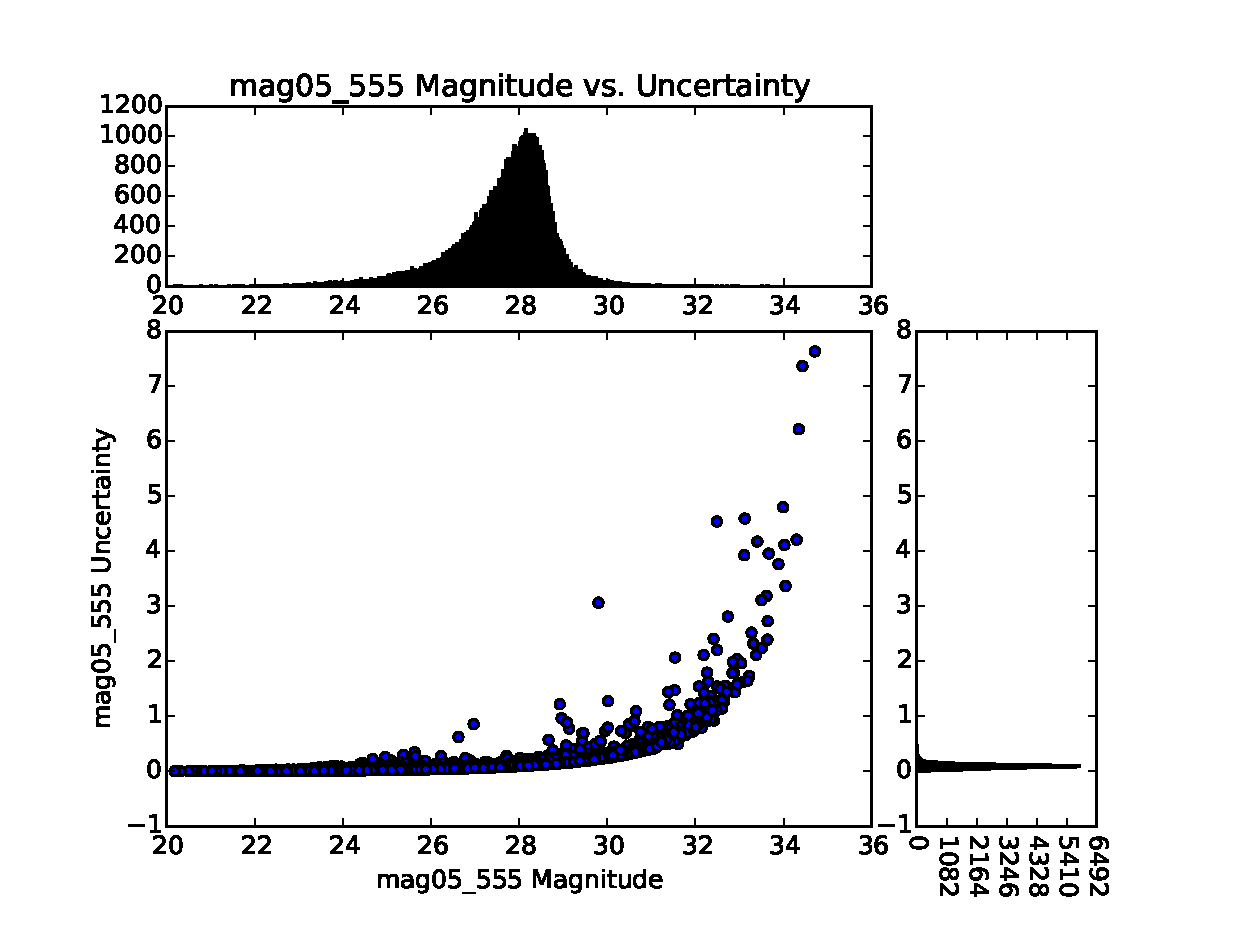
\includegraphics[width=0.5\textwidth]{figs/mag05_555_uncertainty_distribution}\label{fig:mag_unc_broad}}
\hfill
\subfloat[Narrow filter distribution.]{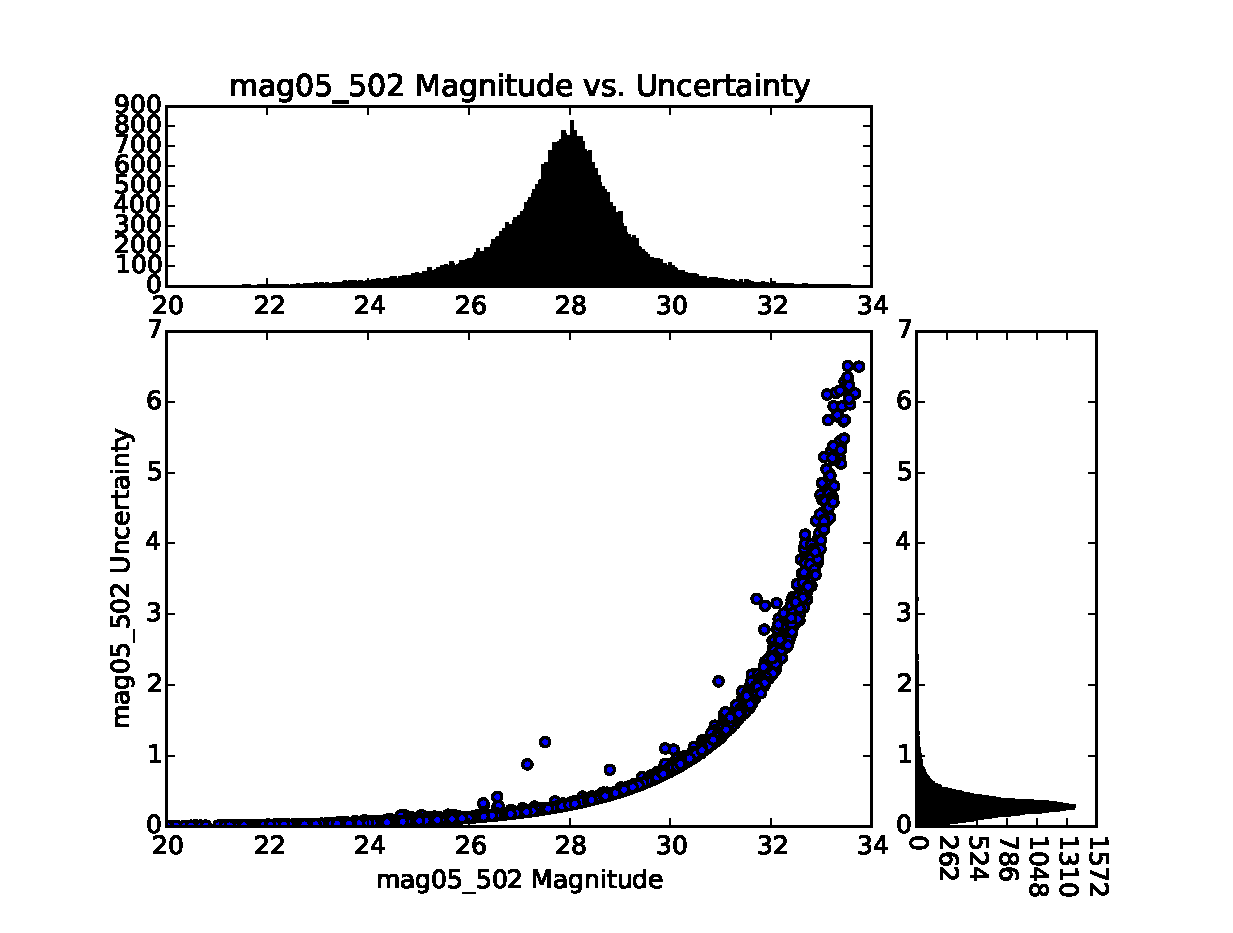
\includegraphics[width=0.5\textwidth]{figs/mag05_502_uncertainty_distribution}\label{fig:mag_unc_narrow}}
\caption{Distribution of magnitudes and uncertainties for objects in the \citet{chandar10} M83 ERS catalog.}
\label{fig:mag_unc}
\end{figure*}

\subsection{Colour Models}
\textbf{Discuss colour models. Figure is broad-band combination with model.}

\begin{figure}
\label{fig:model_colour}
\centering
\includegraphics[width=0.5\textwidth]{figs/data/plot_mag05_555-mag05_814vsmag05_336-mag05_438}
\caption{Colour-colour distribution of $V - I$ and $U - B$ with colour model plotted in pink.}
\end{figure}


\subsection{Published catalogs}

As one check on the results of our analysis, we use previously-published identifications of specific types of objects in M83.
We compiled a `published catalog' by combining the contents of the NASA Extragalactic Database (NED) and
[what does it stand for?] \citep[SIMBAD][]{wenger2000} and then adding the catalogs of Wolf-Rayet stars \citep{kim12} and
red supergiant candidates \citep{williams15}, which did not appear in either database.
NED's focus as an extragalactic database and SIMBAD's focus on Galactic objects mean that their contents overlap but are not identical, 
and this is true of the area surrounding M83. A $3\farcm3$ radius region around the coordinates centered at  ($204.26761\deg, -29.839939\deg$)
contains 1553 NED objects and 1772 SIMBAD objects, of which 1220 are matched with each other at 1\arcsec tolerance.
Although the two services use slightly different naming conventions, with human inspection the matches are generally recognizable as referring
to the same object. Interestingly, the databases do not always report the same object type even when the names are identical.
The differences are reasonable in some cases (a supernova remnant can also be an X--ray source, for example), but not others
(e.g. CXOU J133703.0-294945 is reported as a supernova remnant by SIMBAD and an H${\sc ii}$  region by NED).
A detailed study of the databases is beyond the scope of this work; for the purposes of this analysis, we kept the NED classification
for objects which appeared in both databases.
Objects which appeared in one database but not the other were primarily from recent work \citep[e.g.][]{long2014}, from
older studies likely superseded by newer ones \citep[e.g.][]{larsen1999}, or from studies in which only coordinates relative to
the galaxy centre were given \citep{rumstay83,dvpd83}.

Our final combined catalog has 2425 objects of which 750**check** are in the region covered by the ERS catalog.
The main classes are star clusters (350), X--ray sources (105), supernova remnants (86), H${\sc ii}$ regions (81),  and
radio sources (36).
Nearly every entry in the published catalog had an ERS catalog object within 1\arcsec, and the mean distance between
matched objects was 0\farcs26.
Given the nearly 100-fold difference in object density between the two catalogs, matching based on positions alone may 
result in spurious matches **REF**. *Some discussion of the exact matching procedure is warranted here, and a conclusion
on what the best thing to do is.**


%Outline for data section
%%\begin{enumerate}
%\item Intro to WFC3 ERS dataset
%\item intro to M83: global parameters (distance, size, environment)
%\item existing studies with this dataset (cluster, massive stars, etc)
%\item description of catalog (is there a ref for this??)
%\item anything about these data we don't like/didn't use?

%\end{enumerate}


\section{Methods}
%\section{Clustering Analysis}
As the size of photometric surveys grows, the number of dimensions available for analysis increases.
Clustering methods provide an efficient way of finding structure in high dimensional data by searching for structure in colour spaces that are difficult to visualize. 
Three different techniques were used to cluster the data;
all were implemented using the \textit{sklearn.cluster} Python package version 0.17 \citep{sklearn}. %AKK: please check that this is the right version number
%AKK: is AP in sklearn - or did you implement this yourself?

\subsection{Mean Shift Clustering}
\label{sec:methods_ms}

Mean Shift is a non-parametric clustering technique that is based on probability density function estimates at each point in the data. 
Mean Shift is a very powerful algorithm, but has not been widely used in astronomy. % Find a paper using it
The power of Mean Shift clustering is that the clusters are not confined to a particular shape.
Because Mean Shift moves towards the local mode near the data on which it was initialized, it is useful for estimating the number of significant clusters in a dataset \citep{comanciciu02}.
At each point, the algorithm estimates the density around that point using a small sample of objects surrounding the point.
The algorithm is based on two components: kernel density estimation and density gradient estimation.
The following highlights the major components of the algorithm; for a full description, see \citet{vatturi09}.

The first element of Mean Shift is kernel density estimation. 
The major parameter of Mean Shift is bandwidth, \textbf{\textit{H}}, which is assumed to be proportional to the matrix $\textbf{\textit{H}} = h^2\textbf{\textit{I}}$, with $h>0$ \citet{vatturi09}.
The density estimator for a multivariate density kernel is given by: 
\begin{equation} 
\label{eq:ms_de}
\hat{f}(x) = \frac{c_{k,d}}{nh^d} \sum_{i=1}^n k\Bigg( \norm{\frac{x-x_{i}}{h}}^2 \Bigg)
\end{equation}
where $x_i$ are a set of $n$ independent \textit{d}-dimensional data points, $h$ is the magnitude of the bandwidth matrix, $k(x)$ is the profile of kernel $K(x)$, and $c_{k,d}$ is a normalization constant. %AKK: unclear what difference between $K$ and $k$ is
Estimating the bandwidth correctly is critical to determining the correct number of clusters.
If the bandwidth is too low, the density estimate will be undersmoothed, and Mean Shift will produce many small clusters.
Conversely, if the bandwidth is too large, a small number of large clusters will be detected, resulting in groupings of data that may blur the underlying structure \citet{vatturi09}.

The second element of Mean Shift is density gradient estimation. 
The density gradient is estimated from the gradient of equation~\ref{eq:ms_de} and given by: 
\begin{multline}
\label{eq:ms_dg}
\nabla\hat{f}_{h,K}(x) = \frac{2c_{k,d}}{nh^(d+2)} \Bigg[ \sum_{i=1}^n k^{\prime} \Bigg( \norm{\frac{x-x_{i}}{h}}^2 \Bigg) \Bigg] \\ \Bigg[\frac{\sum_{i=1}^n x_{i}k^{\prime} \Bigg( \norm{\frac{x-x_{i}}{h}}^2 \Bigg)}{\sum_{i=1}^n k^{\prime} \Bigg( \norm{\frac{x-x_{i}}{h}}^2 \Bigg)} - x \Bigg]
\end{multline}
The second term of equation~\ref{eq:ms_dg}, is the Mean Shift, the difference between the weighted mean using $k^{\prime}$ and $x$.
Applying a normal kernel to the Mean Shift, the second term of equation~\ref{eq:ms_dg} becomes: 
\begin{equation} 
\label{eq:ms_sh}
m_{h,K}(x) = \frac{\sum_{i=1}^n x_{i} \exp \Bigg(\norm{\frac{x-x_{i}}{h}}^2 \Bigg)}{\sum_{i=1}^n \exp \Bigg(\norm{\frac{x-x_{i}}{h}}^2 \Bigg)} - x
\end{equation}
$m_{h,K}$ is the Mean Shift, and always points in the direction of largest ascent through the estimated density function \citet{vatturi09}.

Mean Shift clustering involves the iterative application of equation~\ref{eq:ms_sh} to shift the points of a data set towards the direction of the Mean Shift vector.
In each iteration $j$ the points are shifted by: 
\begin{equation}
\label{eq:ms}
x_i^{j+1} = x_i^j + m_{h,K}(x_i^j)
\end{equation}
Shifting the data points by equation~\ref{eq:ms} ensures that when the points converge, the center is the area of highest local density, or density ``mode". 
The density mode can be interpreted as the centre of a significant cluster in the data set and is used to classify the objects that were shifted towards it.
% Add section about bandwidth estimation
% Discuss drawbacks

\subsection{Affinity Propagation Clustering}
\label{sec:methods_ap}

Affinity propagation (AP) is a relatively new clustering technique developed by \citet{frey07}.
The main components are described here; for a full description of the technique, see \citet{frey07}.
AP takes the similarities between the data points as input for clustering, and uses a series of ``messages'' between data points to determine the number of clusters and their centers.
The centres of AP clustering are actual data points, called exemplars; unlike other methods AP does not create average centres for each cluster. 
The first inputs required for AP are the \textit{preferences} of each data point which describe the likelihood of a data point to be chosen as an exemplar.
The preferences are a measure of the similarity between a point \textit{i} and a candidate exemplar \textit{k} defined by: 
\begin{equation}
\label{eq:sim}
s(i,k) = -\norm{x_i - x_k}^2
\end{equation}
Similarity values influence the number of clusters AP identifies, as the larger similarity values are likely chosen as exemplars.
Preference values could be estimated using the median value of the similarities, the minimum value, or randomized to see the effects over various clusterings.
%how does our implementation estimate preference values?

Once the preference value is determined, two messages are computed between all the data points.
The first message is the ``responsibility'' $r(i,k)$, which is sent from point \textit{i} to candidate exemplar \textit{k}:
\begin{equation}
\label{eq:resp}
r(i,k) \leftarrow s(i,k) - max_{k^\prime s.t,  k^\prime \neq k} \{ a(i,k^\prime) + s(i,k^\prime) \}
\end{equation}
Responsibility measures the suitability of point \textit{k} to be an exemplar of point \textit{i} \citet{frey07}, after considering other potential exemplars for point \textit{i}.
The ``availability'', $a(i,k^\prime)$ in Equation~\ref{eq:resp}, is sent from candidate exemplar \textit{k} to point \textit{i} to compute the evidence for how appropriate it would be for point \textit{i} to choose candidate \textit{k} as an exemplar, considering evidence from other points that believe candidate \textit{k} should be their exemplar: %rewrite to avoid implying that data points ``believe'' anything
\begin{equation}
\label{eq:avail}
a(i,k) \leftarrow min\Big\{ 0, r(k,k) + \sum\limits_{i^\prime s.t, i^\prime \notin \{i,k\}} max\{0, r(i^\prime, k)\}\Big\}
\end{equation}

The availabilities of all points are initialized to zero, and the first iteration of responsibilities are set to the input preferences.
Each iteration updates equation~\ref{eq:resp} and equation~\ref{eq:avail} to determine the optimal exemplars for the data.
As the process iterates, for point \textit{i}, the value of \textit{k} that maximizes $a(i,k) + r(i,k)$ identifies \textit{i} as an exemplar if $k=i$, or gives the exemplar of point \textit{i} \citet{frey07}.
In order to ensure that the message passing does not cause numerical oscillations, the messages are damped as they are updated.
The previous message value is multiplied by a damping factor $0 <\lambda<1$, and $1 - \lambda$ multiplied by the update value is added. %AKK: pls clarify second part of this sentence
The damping factor has a default value of 0.5. %AKK: what value did we use? Does it change as the algorithm runs?


\subsection{K-Means Clustering}
K-Means clustering is one of the most widely used clustering methods and has been used to identify a wide range of interstellar and intergalactic objects. % List papers that have done so
It is simple, robust, and easy to implement when analyzing high dimensional spaces, making it a powerful way to analyze multi-band photometric surveys. 
With the k-means algorithm, the number of clusters $K$ must be selected in advance.
K-Means aims to minimize the sum of squares of distances within each cluster given by:
\begin{equation}
\label{eq:km_sos}
J = \sum_{i=1}^N \sum_{k=1}^K \min \big( \norm{x_i - \mu_k}^2 \big)
\end{equation}
The algorithm is initialized by selecting $K$ data points at random and deems these points cluster centres, denoted by $\mu_k$. 
Each point in the data set $x_i$ is then assigned to a cluster centre by finding the centre to which the least-squares distance is the smallest.
The algorithm iterations continue with the centres being re-calculated by taking the average position of all the points in each cluster and reassigning each point to the nearest cluster centre.
The stopping criterion is that the centres do not change after two consecutive iterations \citep{sanchez-almeida13}. %change by how much? why are we citing this particular paper?

% Discuss drawbacks
% K-Means requires the number of clusters to be inputed by the user. 
% This posses a challenge for high dimentional data, as the number of clusters cannot be estimated by visual inspection. 

\section{Analysis}
% Analysis section
This section will outline colour construction, the clustering process, and the selection of the optimal clustering for each colour combination.
Each colour combination was clustered using the same process, and in two and three dimensions.

\subsection{Colour Selection}

Observations in 10 bands allow the generation of 45 different colours, but not all of these colours are likely to be useful in characterizing components of the galaxy.
Since the average survey consists of four filters, different combinations of four filters were used to construct colours for clustering. 
Due to the large number of filters available in the ERS data, the combinations had to be narrowed down to a reasonable set.
Two types of colour combinations were created: combinations of all broad band filters, and combinations with one narrow band and three broad bands.
Additionally, two and three dimensions were considered for clustering, in order to maximize the use of the data in an average survey.

\subsubsection{Broad Band Combinations}

\textbf{PB: Should we explain what kind of objects we hope to find in these combos?}

The first type of combination was comprised of the broad band filters: F336W (U), F438W(B), F555W(V), and F814W(I).
The F225W (UVW) filter was not included in this set as it is not a standard filter most surveys.
Additionally, the $U - I$ colour was not used in the analysis because it was determined that this colour was not physically meaningful.
This is because it is unlikely that an object would emit a detectable reading in both these bands due to their distance from one another in wavelength.
Using the four filters, the broad band colour combinations created can be found in Table~\ref{tab:BBcolours}.
These combinations were created in order to remove any obvious correlation between the colours that could occur by the inclusion of the same band in both colours.

\begin{table*}
\centering
\caption{Broad band colour combinations and the number of objects detected in each colour, and in each combination, with uncertainties less than $0.2$.}
\label{tab:BBcolours}
\begin{tabular}{lllllll}
\hline\hline
Colour 1 & Objects & Mean Uncertainty & Colour 2 & Objects & Mean Uncertainty & Combined Objects \\
\hline
$U - B$ &  33523 & 0.1606 mag & $V - I$ &  57935 & 0.1334 mag & 28931\\
$U - V$ &  33692 & 0.1429 mag & $B - I$ &  41413 & 0.1590 mag & 28931\\
$B - V$ &  48660 & 0.1456 mag & $ - $ & $ - $ & $ - $ & $ - $ \\
\hline
\end{tabular}
\end{table*}

\subsubsection{Narrow Band Combinations}

\textbf{PB: Should we explain more about why we choose to do Broad - Narrow? And what objects we hope to find in these combos?}

The second set of combinations included the narrow band filters: F373N ($O_{2}$), F487N ($H\beta$), F502N ($O_{3}$), F657N ($H\alpha$), and F673N ($S_{2}$).
In addition, the broad band F225W (UVW) was included in this set to ensure its data was included in the analysis. 
Colours were created with the narrow bands by pairing them with the broad bands that covered them in wavelength space.
These colours were created in order to reduce the number of possible combinations that could be used for analysis.
The second colour in each combination was created from two broad bands that did not overlap the first colour in wavelength space.
Table~\ref{tab:NBcolourcombos} lists the narrow band colour combinations used for analysis.
The number of objects in the narrow band combination, with the exception of the $H\alpha$ band, is significantly lower than the broad band combinations.
These combinations were useful for analysis as their distributions were not as dense as the broad bands, and the clustering algorithms were able to detect interesting structure within them.
Making colours out of a combination of broad and narrow bands ensure that the objects clustered in these bands are physically meaningful, as it is likely that the object would emit in the broad band that contains the narrow band. \textbf{Not sure if that is a reason why we chose to construct them that way}.

\begin{table*}
\centering
\caption{Narrow band colour combinations and the number of objects detected in each colour, and in each combination, with uncertainties less than $0.2$.}
\label{tab:BBcolours}
\begin{tabular}{lllllll}
\hline\hline
$Narrow - Broad$ & Objects & Mean Uncertainty & $Broad - Broad$ & Objects & Mean Uncertainty & Combined Objects \\
\hline
$UVW - U$ &  14977 & 0.1539 mag & $B - V$ &  48660 & 0.1456 mag & 14943 \\
$ - $ & $ - $ & $ - $ & $B - I$ &  41413 & 0.1590 mag & 14095 \\
$ - $ & $ - $ & $ - $ & $V - I$ &  57935 & 0.1334 mag & 14098 \\
\hline
$U - O_{2}$ & 8675 & 0.1504 mag & $B - V$ &  48660 & 0.1456 mag & 8657 \\
$ - $ & $ - $ & $ - $ & $B - I$ &  41413 & 0.1590 mag & 8558 \\
$ - $ & $ - $ & $ - $ & $V - I$ &  57935 & 0.1334 mag & 8559 \\
\hline
$B - H\beta$ & 13269 & 0.1493 mag & $V - I$ &  57935 & 0.1334 mag & 13147 \\
\hline
$O_{3} - V$ & 14644 & 0.1418 mag & $U - B$ &  33523 & 0.1606 mag & 13390 \\
\hline
$H\alpha - I$ & 59465 & 0.1495 mag & $U - B$ &  33523 & 0.1606 mag & 28920 \\
$ - $ & $ - $ & $ - $ & $U - V$ &  33692 & 0.1429 mag & 29060 \\
$ - $ & $ - $ & $ - $ & $B - V$ &  48660 & 0.1456 mag & 41317 \\
\hline
$S_{2} - I$ & 25185 & 0.1535 mag & $U - B$ &  33523 & 0.1606 mag & 14577 \\
$ - $ & $ - $ & $ - $ & $U - V$ &  33692 & 0.1429 mag & 14586 \\
$ - $ & $ - $ & $ - $ & $B - V$ &  48660 & 0.1456 mag & 18882 \\
\hline
\end{tabular}
\end{table*}

\subsubsection{Number of Dimensions}
Due to the high number of bands available in the ERS data, the number of dimensions available to cluster was very high.
Limiting the number of band combinations through the system outlined above helped reduce the number of dimensions.
However, in addition to the two dimensional combinations, clustering in three dimensions was investigated.
Three dimensional colour combinations were created based on the combinations listed in Table~\ref{tab:BBcolours} and Table~\ref{tab:NBcolourcombos}.
In the broad band combinations, three dimensional colour spaces were created by making colours with a common band, either B or V.
These bands were selected in order to avoid creating the $U - I$ colour.
\textbf{PB: Not sure if this next sentance explains why we chose to use a common band clearly. Just trying to say that the colours could be subtracted to transform back into the two dimensional space.}
A common band was used in all colours in order to create a three dimensional space that of colours that could be transformed back into the original two dimensional space. 

In the narrow band combinations, the three dimensional colour spaces were created by making colours with the narrow band common between them.
Similar to the broad band spaces, these combinations could be transformed into the original two dimensional space, and act as an extension of the two dimensional distribution.

Clustering in three dimensions increased the complexity of the distribution, creating more information for the clustering algorithms to use.
However, limiting the dimensionality of the problem to three allowed the analysis to stay within the constraints of a common survey.
A space of up to 45 dimensions could have been created, but that space would not be reasonable for the analysis of a common survey.

\subsection{Clustering Process}
Clustering was performed using all methods for each colour combination. 
The following process allowed the investigation of the effect of all paramters on each clustering technique, leading to the selection of an optimal clustering.

\subsubsection{Meanshift}
Mean-Shift clustering was performed first by estimating the bandwidth paramter with the $estimate-bandwidth$ function in $scikit-learn$. \textbf{How do we cite this package?}
This function estimates the bandwidth parameter based on the distances between points in the dataset, and determines if the distribution has high or low variance.
Following the initial clustering, a the bandwidth was varried and the clustering was performed again with bandwidth values on intervals of $\pm 0.1$ from the estimated bandwidth value.
Varying the bandwidth revealed how sensitive a combination was to the parameter.
If a combination was very sensitive to bandwidth, then the number of clusters that meanshift would predict would vary greatly over a small range of bandwidth values.
This type of combination usually resulted in poor segmentation, as the algorithm would not converge on a number of clusters. 
However, sensitivity could also be the result of the starting bandwidth estimate.
If the original estimate was in an unstable bandwidth interval, then the hierarchy would reflect that, and the testing of multiple bandwidth values could result in convergence.

\subsubsection{Affinity Propagation}
Affinity Propagation clustering was performed after Meanshift. 
The first clustering was run using the preference estimations outlined in Section 3. \textbf{how to referene section}.
The preferences were set to the median and the minimum value of the similarities, and the damping factor was kept at the default value of $0.5$.
This resulted in a segmentation with over 100 clusters in multiple colour combinations.
The preferences were then set to 10\% of the number of objects in the data set, and the damping factor was set at $0.95$.
With these parameters, the clusterings varried significantly over differnet colours. 
The clusterings were repeated to try and reveal a trend in the parameters, but the algorithm was too sensitive for this size of dataset.
Following the initial tests of Affinity Propagation, it was determined that this clustering method was not effective.
Due to the number of computations required for the calculation of the messages passed between points on each iteration, the algorithm was very sensitive to the input parameters, and did not produce meaningful clusterings.
The algorithm is effective for small and medium sized datasets, and was able to create some reasonable clusters when the uncertainty limit was set at $0.1 mag$, which reduced the number of objects significantly. 
After multiple clusterings, a systematic way of determine the correct number of clusters could not be determined, and the algorithm was not used further.

\subsubsection{K-Means}
K-Means clustering was performed last.
The first clustering was performed using the number of clusters determined from the initial clusterings by Meanshift.
Next, K-Means was performed with $K = \pm 4$ from the original clustering.
This method of clustering was similar to the Meanshift approach, as it revealed how the dataset reacted to different values of $K$.
K-Means was the most efficient algorithm of the three, as it produced clusterings quickly, and always produced clusters of reasonable size.

\subsection{Selecting the Optimal Clustering}
Determining the optimal clustering was the most difficult task of the analysis.
Selecting the optimal clustering can often seem arbitrary, as no ``right" answer is obvious.
In order to determine the optimal clustering, a variety of metrics and statistics were calculated to evaluate each cluster.
Additionally, the relationships between a variety of clustering parameters were investigated to try and determine where they indicated the optimal clustering.
Since the performance of the algorithms was directly related to the parameters used as input, those relationships were critical for selecting the clustering.
The objects in each cluster were then found in the white-light image of M83, to determine if there was a relationship between the objects assigned to the same cluster and their spatial position.
Finally, colour models were created and imposed on the cluster distribution to determine if the segmentation agreed with a model. \textbf{Need more on why the models were used}.

\subsubsection{Silhouette Score}
The silhouette score is a metric used to describe the compactness of a cluster in a given clustering and is calculated as an average of all samples in a clustering.  
The silhouette score is given by:

\begin{equation}
\label{eq:ss}
Silhouette Score = \frac{b - a}{\textit{max}\big(a, b\big)}
\end{equation}

where $a$ is the mean intra-cluster distance, and $b$ is the distance between a point and the nearest cluster that point is not a member of.
The score was used in two ways.
First, the average score was calculated for a given clustering.
This calculated the average score across all data in the sample.
Next, the average score for each cluster was computed.
The average cluster score evaluates the strength of a given cluster within a clustering.
This metric allowed each cluster to be evaluated individually, and revealed which clusters were responsible for the average score of the clustering.
Additionally, the average score allowed seemingly arbitrary clusters to be evaluated.
If the segmentation did not seem meaningful, the average score would reveal if the cluster was isolated and compact.
This revealed the significance of clusters that could have been viewed as noise or outliers. \textbf{This section needs more explaination}.

\textbf{Struggling to explain why that is how the score works}. 
Ideally, the silhouette score for the entire clustering should peak near the center of the distribution indicating the optimal clustering. 
High scores where the number of clusters is low often do not reflect the structure of the distribution, while high numbers of clusters are often imposed on the data as a result of the specified parameters.
This is often not the case, as seen in Figure~\ref{fig:sscore}, which shows the distribution of the silhouette score against the number of clusters.
For the K-Means clusterings, the score does not peak in the center of the distribution.
Instead of selecting the clustering with the highest score, the optimal clustering is found where the relation begins to elbow; between 4 and 5 clusters.
This clustering is selected because any increase in $K$ after this point does not affect the score, and does strengthen or weaken the clustering.
This means that the algorithm has found the balance between the natural clusters in the distribution and artificially segmenting the data.

\begin{figure}[H]
\centering
\includegraphics[width=\linewidth]{figs/methods/silhouette_score_relation}
\caption{Distribution of the silhouette score as a result of the number of clusters imposed for the $UVW - U$ and $V - I$ colours. The \textit{blue} points are the scores of Meanshift clustering, \textit{red} points are scores of K-Means.}
\label{fig:sscore}
\end{figure}

The distribution of score as a result of the Meanshift algorithm does not follow the same pattern.
The silhouette score was not as successful at describing the strength of Meanshift clusterings as Meanshift often created one large cluster and several smaller ones, which is not considered strong by the score.
In order to determine the optimal Meanshift clustering, other relationships were investigated.

\subsubsection{Cluster Statistics}
Various statistics were calculated to help describe the similarity between the objects in a given cluster.
The standard deviation and average colour was calculated for each colour, and each cluster within a clustering. 
These metrics helped describe the distribution of the objects in the colour-colour space within a cluster. 
Clusters that had large standard deviations were viewed as too dissimilar to be a meaningful cluster, and clusters whose averages varried significantly from the cluster centers were disgarded.

\textbf{I'm not sure that this paragraph describes why we calculated the fractional size}.
The fractional size of each cluster was also calculated and described the distribution of objects between clusters.
If a clustering segmented the objects into a large cluster followed by several smaller ones, the clustering was investigated further, as this segmentation could mean one of two things. 
This type of clustering could be a result of the identification of interesting objects, in which case the clustering algorithm was able to identify the objects and place them in the same cluster.
However, this type of clustering could also be a result of the underlying distribution of the data, as the clustering techniques are largely drawn to areas of high density.
If this is the case, the clustering only created the smaller clusters as a result of the parameters imposed on the clustering.

\subsubsection{Parameter Relationships}
In addition to metrics, the relationships between various parameters were investigated to determine how the each clustering method behaved.

Each K-Means clustering was checked by plotting the sum-of-squares value for each value of $K$.
Figure~\ref{fig:inertia} shows the inertia distribution for the $H\beta - B$ vs. $V - I$ colour.
As $K$ increases, the inertia value decreases as the inertia value represent the total distance between the total distance between the points of each cluster.
The value decreases with $K$ as the total distance in each cluster decreases as more clusters are introduced.
This distribution was used to check the clustering and ensure that the clusterings were successful.

\begin{figure}[H]
\centering
\includegraphics[width=\linewidth]{figs/methods/inertia_plot}
\caption{Distribution of the inertia as a result of the number of clusters for the $H\beta - B$ and $V - I$ combination.}
\label{fig:inertia}
\end{figure}

Following the inertia test, the cluster centers were tested by running K-Means for 40 trials with the same value of $K$.
This test was run to determine if the clusterings were stable as K-Means is initiallized randomly, and the clusters produced can depend on the starting position.
Figure~\ref{fig:cen_test} shows the result of the three dimensional clustering test for the $U - O_{2}$ and $B - V$ combination.

\begin{figure}[H]
\centering
\includegraphics[width=\linewidth]{figs/methods/3_cl_cluster_centers}
\caption{Distribution of the cluster center as a function of the trial number for the three dimensional $U - O_{2}$ and $B - V$ combination with $K=3$. The left panel plots the centers in the $U - O_{2}$ colour, and the right panel plots the centers in the $B - V$ colour. Each line of dots represents a single cluster, and the colours represent the cluster number.}
\label{fig:inertia}
\end{figure}

It is clear that each initialization found different clusters first as the colours in each line are not constant. 
Despite the random initialization the final cluster centers did not change.
This distribution of cluster centers represents a strong clustering. 
If the cluster centers vary across multiple initializations of K-Means, the clustering would not be reliable, and the combination would not be considered for analysis.

The behavior of the bandwidth parameter was investigated for each Meanshift clustering.
Figure~\ref{fig:bad_ms} shows the relation between the score and number of clusters for the three dimensional $U - O_{2}$ and $B - I$ combination.
The blue dots represent the Meanshift clusterings.

\begin{figure}[H]
\centering
\includegraphics[width=\linewidth]{figs/methods/silhouette_score_bad_ms}
\caption{Distribution of the silhouette score as a result of the number of clusters imposed for the three dimensional $U - O_{2}$ and $B - I$ combination. The \textit{blue} points are the scores of Meanshift clustering, \textit{red} points are scores of K-Means.}
\label{fig:bad_ms}
\end{figure}

It is clear that an optimal clustering cannot be determined from this relation, as the score decreases linearly with the number of clusters Meanshift predicts.
The Mean-Shift scores do not follow a similar distribution as K-Means, as the accuracy of Meanshift is related to the bandwidth parameter, seen in Figure~\ref{fig:bwscore}.
The optimal Mean-Shift clustering was chosen by finding the bandwidth where the relation between the bandwidth and number of clusters reached an elbow, or where the relation between bandwidth and silhouette score elbowed.
In both panels of Figure~\ref{fig:bwscore} that the bandwidth parameter predicts five clusters.
Both distributions elbow at the same bandwidth interval, maximizing the score and predicting the same number of clusters for bandwidth valeus following the elbow.
The bandwidth parameter was the primary indicator of the optimal Meanshift clustering.
If a trend could not be found with the bandwidth parameter, then the silhouette score and number of clusters was investigated.

\begin{figure}[H]
\centering
\includegraphics[width=\linewidth]{figs/methods/meanshift_parameters}
\caption{Distribution of the silhouette score as a function of bandwidth, and the distribution of the number of clusters as a function of bandwidth.}
\label{fig:bwscore}
\end{figure}
\section{Results}
% Results section

The section will outline the major results of the clustering. 
It is focused on the broad band clustering, and two combinations from the narrow band colours.
The first narrow band combination is the most successful narrow band clustering, and the second is the least successful.
A complete discussion of all the combinations can be found in Appendix 1 \textbf{Make appendix here}.

% BROAD BAND CLUSTERINGS ----------------------------------------------
\subsection{Broad - Broad Band Combinations}
Table~\ref{tab:BBcolours} lists the broad band combinations that were clustered. 
In both two and three dimensions, the $U - B$ and $V - I$ combination was clustered more effectively than the $U - V$ and $B - I$ combination, and will be the combination used for discussion.

\subsubsection{2-Dimensions}
The two dimensional clustering was successful in identifying features within the distribution, however, it's segmentation was not as strong as the three dimensional clustering. 
% Broad band table
%\begin{landscape}
\begin{table*}
\centering
\caption{Summary of $U - B$ and $V - I$ combination two dimensional clusterings.}
\label{tab:BBclustering}
\begin{tabular}{llllllllllll}
\hline\hline
Method & Clusters & Parameters & Score & Cluster 1 & Cluster 2  & Cluster 3 & Cluster 4 & Cluster 5 & Cluster 6 & Cluster 7 & Cluster 8\\
\hline
K-Means & 3 & $K = 3$ & 0.4413 & 2215 & 7892 & 18824 & $ - $ & $ - $ & $ - $ & $ - $ & $ - $ \\
K-Means & 4 & $K = 4$ & 0.3741 & 2590 & 12924 & 2034 & 11383 & $ - $ & $ - $ & $ - $ & $ - $ \\
K-Means & 5 & $K = 5$ & 0.3577 & 7541 & 1513 & 5472 & 2298 & 12107 & $ - $ & $ - $ & $ - $ \\
K-Means & 6 & $K = 6$ & 0.3271 & 986 & 1618 & 5237 & 8373 & 8149 & 4568 & $ - $ & $ - $ \\
K-Means & 7 & $K = 7$ & 0.3254 & 4512 & 2371 & 999 & 6862 & 7283 & 1047 & 5857 & $ - $ \\
K-Means & 8 & $K = 8$ & 0.3186 & 2733 & 4437 & 5737 & 5091 & 6705 & 2455 & 684 & 1089 \\
Meanshift & 8 & $h = 0.4000 $ & 0.4236 & 25308 & 2518 & 48 & 6 & 57 & 917 & 1 & 76 \\
Meanshift & 5 & $h = 0.4500 $ & 0.3981 & 28074 & 533 & 9 & 1 & 314 & $ - $ & $ - $ & $ - $ \\
Meanshift & 5 & $h = 0.5000 $ & 0.3962 & 28129 & 487 & 9 & 305 & 1 & $ - $ & $ - $ & $ - $ \\
Meanshift & 5 & $h = 0.5500 $ & 0.4037 & 27927 & 706 & 9 & 1 & 288 & $ - $ & $ - $ & $ - $ \\
\hline
\end{tabular}
\end{table*}
%\end{landscape}
Table~\ref{tab:BBclustering} summarzies the results of the two dimensional clusterings.
This table lists the parameters that produced the clusterings, and the number of objects in each cluster.

\paragraph{K-Means}
The optimal clustering selected was at $K=5$ (Figure~\ref{fig:BB2dKM5} as it is the point where the score begins to plateau.
K-Means performed more effectively than Meanshift in 2-dimensions.
K-Means was able to identify the branch of red $U - B$ objects at low values of $K$.
As $K$ increased, the algorithm was also able to identify a group of objects that are red in $V - I$, and blue in $U - B$. 

\begin{figure}[H]
\centering
\includegraphics[width=\linewidth]{figs/broad/kmeans_color_5cl_mag05_555-mag05_814vsmag05_336-mag05_438}
\caption{Colour-Colour distribution of the $U - B$ and $V - I$ colours, clustered using K-Means with $K=5$. The colour of each point corresponds to the cluster the point was assigned to. Cluster numbers can be seen in the legend.}
\label{fig:BB2dKM5}
\end{figure}

The boundaries of each cluster approximately represent integers in each colour, and identify groups of objects that are relatively blue and red, seperating them from objects with extremes of either colour.
\textbf{Discuss statistics here}
The clusters trace sections of the modelled colours. 
The centers of clusters 2 and 5 line up well with the models, indicating that these clusters could be representative of different ages of objects in this distribution.
\textbf{Not sure if that was the right implication or if there is something else to their alignment}. 

\paragraph{Meanshift}
The optimal Meanshift clustering was selected as the point where the bandwidth converged, and can be seen in Figure~\ref{fig:BB2dMS5}.
Its bandwidth was $h=0.6$, which produced five clusters.

\begin{figure}[H]
\centering
\includegraphics[width=\linewidth]{figs/broad/meanshift_color_5cl_mag05_555-mag05_814vsmag05_336-mag05_438}
\caption{Colour-Colour distribution of the $U - B$ and $V - I$ colours, clustered using Meanshift with $h=0.6$ producing five clusters. The colour of each point corresponds to the cluster the point was assigned to. Cluster numbers can be seen in the legend.}
\label{fig:BB2dMS5}
\end{figure}

This clustering was not as strong as K-Means, as it failed to identify the branch of red objects (cluster 2 in Figure ~\ref{fig:BB2dKM5}) that is a major feature of the distribution.
Additionally, the clusters and their centers do not align with the model colours, indicating that Meanshift was unable to identify different segments of the stellar lifecycle.
\textbf{Add cluster statistics here}.

\paragraph{Clustering Comparison}
Figure~\ref{fig:BB2dMSKMcomp} shows the comparison between the two optimal clusterings.

\begin{figure}[H]
\centering
\includegraphics[width=\linewidth]{figs/broad/kmeans-5cl_mag05_555-mag05_814_vs_meanshift-5cl_mag05_-mag05__mag05_-mag05__2ddim_compare}
\caption{Comparison of object cluster assignment between Meanshift and K-Means clusterings.}
\label{fig:BB2dMSKMcomp}
\end{figure}

The axes are the respective clusterings, and the size of the bubble is related to the number of objects that belongs to both clusterings.
It is clear that there is little agreement between the cluster assignment between the two methods. 
Cluster 2, the red branch of objects, is the only cluster where a significant portion of objects were assigned to the same cluster. \textbf{Implication}
K-Means distributes objects far more evenly between clusters, and creates more meaningful segmentation as seen in Figure~\ref{fig:BB2dKM5}.
Due to this comparison, the K-Means segmentation was selected as the optimal clustering for this combination, and was used for the completion of the results.

\paragraph{M83 Locations}

The clusters from the two dimensional clustering show distinct locations in M83.
The branch of red $U - B$ objects found in Cluster 2 of Figure~\ref{fig:BB2dKM5} are objects that lie loosly around the spiral arms.
These objects are generally not found in the concentrated regions of the arms, and lie to the left and right of these areas.
On the whitelight image, these objects appear to be isolated, dim point sources that could be lying behind clouds of dust, in the back of the galaxy, or on their own outside the arm.
\textbf{PB: What could these objects actually be? Young star clusters, clouds, background sources/galaxies?}

The branch of red $V - I$ objects found in Cluster 4 of Figure~\ref{fig:BB2dKM5} are objects that lie primarely in the dense regions of the spiral arms, with a few objects lying in the nucleus, and in the region south of the nucleus.
These objects also appear to be quite dim point sources, or no detection in the whitelight image.
This could mean that the objects are some form of cloud, nebula, or background galaxy. 
These objects are interesting as their $V - I$ colour stretches to values over 3, indicating very red emission. \textbf{PB: is this all true...}

Despite the seemingly arbitrary segmentation of clusters 1 and 3, the objects seem to inhabit different regions of M83.
These two clusters generally trace each others location in the galaxy. 
Cluster 1 is generally confined to the denser regions of the arms, while cluster 3 fills in the areas between the objects in cluster 1.
Cluster 1 objects appear to be bright point sources on the whitelight image, while cluster 3 objects are dim or non-existant.
\textbf{PB: what could these objets be?}.

Interestingly, despite their difference in colour, cluster 5 also traces clusters 1 and 3 around the galaxy.
Cluster 4 objects stay mainly concentrated in the spiral arms, filling in the dense area in the interarm regions.
Cluster 4 objects are not as apparent in the interarm region as clusters 1 and 3, but still appear in denser areas. \textbf{PB: what could these objects be?}

\subsubsection{3-Dimensions}
Three dimensional clustering was performed with the colour combinations found in Table~\ref{tab:BB3dcolours}.

\begin{table*}
\centering
\caption{Broad band colour combinations in three dimensions}
\label{tab:BBcolours}
\begin{tabular}{lllll}
\hline\hline
Base Colour 1 & Base Colour 2 & Colour 1 & Colour 2 & Colour 3 \\
\hline
$U - B$ & $V - I$ & $U - B$ & $B - V$ & $B - I$ \\
$U - V$ & $B - I$ & $U - V$ & $B - V$ & $V - I$ \\
\hline
\end{tabular}
\end{table*}

Both K-Means and Meanshift identified interesting clusters in three dimensions.

\paragraph{K-Means}
Similar to two dimensions, K-Means was able to identify objects that were in specific regions of the colour space.
The optimal K-Means clustering was found at $K=4$ (Figure~\ref{fig:BB3dKM4}), as the score peaked, and the red branch of objects was identified. \textbf{What is the significance of the red branch?}
Figure~\ref{fig:BB3dKMproj} displays the projection of the three dimensional clustering into each of its two dimensional components. 
It is clear that the three dimensional clustering was driven by the $B - I$ vs. $U - B$ distribution, as the clusters were almost completely seperated in that space.
The clusters overlapped extensively in the $B - V$ vs. $U - B$ space. \textbf{PB: Do you know why this would be? Would it be from the range of colour in the B-I dimension?}
This could be a result of the colour distribution in the $B - I$ space, as the range of object colour in this dimension is much larger than in the $B - V$ colour.
This relationship was found through all colour combinations.

\begin{figure*}
\centering
\subfloat[$U - B$ vs. $B - V$ Distribution.]{\includegraphics[width=0.5\textwidth]{figs/broad/kmeans_3d_projection_4cl_mag05_336-mag05_438vsmag05_438-mag05_555}\label{fig:BB3dKMprojBV}}
\hfill
\subfloat[$U - B$ vs. $B - I$ Distribution.]{\includegraphics[width=0.5\textwidth]{figs/broad/kmeans_3d_projection_4cl_mag05_336-mag05_438vsmag05_438-mag05_814}\label{fig:BB3dKMprojBI}}
\caption{$U - B$ vs. $B - V$ and $B - I$ projections from three dimensional clustering.}
\label{fig:BB3dKMproj}
\end{figure*}

\begin{figure}[H]
\centering
\includegraphics[width=\linewidth]{figs/broad/kmeans_3d_4cl_mag05_336-mag05_438vsmag05_438-mag05_555vsmag05_438-mag05_814}
\caption{Colour-Colour-Colour distribution of the $U - B$, $B - V$, and $B - I$ colours, clustered using K-Means with $K=4$. The colour of each point corresponds to the cluster the point was assigned to. Cluster numbers can be seen in the legend.}
\label{fig:BB3dKM4}
\end{figure}

The three dimensional clustering illustrates how the algorithm is able to identify two distinct branches of objects beyond the dense center of the distribution.
Cluster 4 is a branch of objects that is quite red in both the $U - B$ and $B - V$ colours, but is neutral in the $B - I$ colour.
Cluster 3 is a branch of objects quite blue in the $U - B$ colour, but red in the other two. \textbf{what is the implication of this?}
The algorithm then segments the dense section of the distribution between the bluer and redder objects in the $B - V$ and $B - I$ colours.
These two clusters are not ideal, as the dense portion of the distribution could be argued as the same cluster. 
However, at $K = 3$, the branches were not identified, so the segmentation of the dense region is necessary.
The clusters projected into the base colours can be seen in Figure~\ref{BB3dKM4base}, where the branches of objects are clearly identified.
\textbf{Add cluster statistics table}

\begin{figure}[H]
\centering
\includegraphics[width=\linewidth]{figs/broad/kmeans_base_color_4cl_mag05_336-mag05_438vsmag05_555-mag05_814}
\caption{Colour-Colour distribution of the $U - B$, and $V - I$ colours, projected from the three dimensional clustering using K-Means with $K=4$. The colour of each point corresponds to the cluster the point was assigned to. Cluster numbers can be seen in the legend.}
\label{fig:BB3dKM4base}
\end{figure}

Similar to the two dimensional clustering, the cluster centers of clusters 1, 2, and 4, match the model colours predicted.
The red branch of objects traces the older stellar population, while clusters 1 and 2 trace the young and intermediate ages of the population.
Cluster 3 is positioned near the loop in the stellar model, however there is a disagreement in the $U - B$ colour.
\textbf{Any other implications of the model matching?}

\paragraph{Meanshift}

Meanshift was also able to produce interesting clusters in three dimensions. 
The optimal clustering was chosen at $h=0.75$ which produced 4 clusters.
This clustering was the peak score, but was not the number of clusters for most intervals of bandwidth.
Most bandwidth values predicted 6 clusters, however, the score and cluster seperation at those intervals was poor.
Figure~\ref{fig:BB3dMS4} shows the three dimensional clustering at $h=0.75$.

\begin{figure}[H]
\centering
\includegraphics[width=\linewidth]{figs/broad/meanshift_3d_4cl_mag05_336-mag05_438vsmag05_438-mag05_555vsmag05_438-mag05_814}
\caption{Colour-Colour-Colour distribution of the $U - B$, $B - V$, and $B - I$ colours, using Meanshift with $h=0.75$. The colour of each point corresponds to the cluster the point was assigned to. Cluster numbers can be seen in the legend.}
\label{fig:BB3dMS4}
\end{figure}

Meanshift identified two groups of objects that lie above the dense area of the distribution in Figure~\ref{fig:BB3dMS4}.
Figure~\ref{fig:BBMS3d4p} shows the projection into the original space, where the cluster location is easier to identify.
The clustering identified two groups of ojbects which are quite red in the $V - I$ colour, but have different $U - B$ colours. 
Cluster 4 is blue in the $U - B$ colour while Cluster 2 is redder.
This identification highlights Meanshift's ability to find outliers in the distribution, as it does not pick out the large branch of objects that are red in $U - B$.
However, these two clusters combined only hold 3\% of the objects used for clustering.
These clusters would have been considered insignificant, however, they are also found at $h = 0.55$.
This means that the clusters are identified at various bandwidth intervals, which means they are likely significant clusters. 
\textbf{Add cluster statistics table}

\begin{figure}[H]
\centering
\includegraphics[width=\linewidth]{figs/meanshift_base_color_4cl_mag05_336-mag05_438vsmag05_555-mag05_814}
\caption{Colour-Colour distribution of the $U - B$, and $V - I$ colours, projected from the three dimensional clustering using Meanshift with $h=0.75$. The colour of each point corresponds to the cluster the point was assigned to. Cluster numbers can be seen in the legend.}
\label{fig:BB3dMS4p}
\end{figure}

\paragraph{Cluster Comparison}
Comparing the two clusterings resulted in a similar comparison to the two dimensional clustering.
No significant distribution between clusters was apparent, and all the K-Means clusters were placed in Cluster 1 of the Meanshift clustering.
However, since the three dimensional Meanshift segmentation was more meaningful than the two dimensional clustering, it was kept for further analysis.

\paragraph{M83 Locations}

In the K-Means clustering (Figure~\ref{fig:BB3dKM4p}), clusters 4 and 3 follow similar patterns found in two dimensions.
These clusters are the red $U - B$ branch of objects and the red shelf of $V - I$ objects that span the whole range of $U - B$ colour.
Cluster 4 objects are generally located in the spiral arms, but their location is not concentrated, and they are fanned across the entire width of the arms.
This is in agreement with the cluster that identified the red branch in two dimensions, however, three dimensions seems to include more objects that could be considered redder than the rest of the distribution.
Cluster 3 objects trace cluster 4, but are in the dense regions of the spiral arms, and do not fan out. \textbf{PB: What could these be?}
Clusters 1 and 2 in three dimensions do not provide the same detail as two dimensions as they lump all the objects in the center of the distribution into two groups.
There are no patterns in object location in these two clusters.

The outlying clusters identified by Meanshift in three dimensions are located in interesting areas of M83.
There is almost no overlap between the locations of the objects in these two groups. 
Cluster 2 objects are fanned out through the spiral arms, and in the core of the galaxy.
These objects appear to be dim point sources on the whitelight image, and could be background objects. 
Cluster 4 objects are also found in the spiral arms, however, they are almost only concentrated in the dense areas. 
These objeccts are found in the same regions of the arms as cluster 2, but they are not close to one another. 
This could indicate that these two classes of objects are different physical objects in M83. \textbf{Not sure if this is the right result of their locations}
Lastly, cluster 3, a single object, does not appear to be a meaningful object. It does not seem to be detected in the whitelight image, as it is in an area without a clear, independent point source.
Since this object has very blue colours, it is not clear what it could be, and may be noise. \textbf{Not sure if this is true!}

\subsubsection{Two and Three Dimension Comparison}
Figure~\ref{fig:BB2a3dKMcomp} shows the comparison between the two and three dimensional clusterings.

\begin{figure}[H]
\centering
\includegraphics[width=\linewidth]{figs/broad/kmeans-4cl_mag05_336-mag05_438_vs_kmeans-5cl_mag05_555-mag05_814_mag05_336-mag05_438_3a2ddim_compare}
\caption{Comparison of object cluster assignment between K-Means in two dimensions and K-Means in three dimensions.}
\label{fig:BB2dMSKMcomp}
\end{figure}

There is significant overlap in each of the five clusters from the two dimensional clustering.
This shows agreement between the two clusterings for which objects belong in the same cluster. 
It is difficult to compare clusterings with a different number of clusters, but it is clear that Cluster 2 in Figure~\ref{fig:BB3dKM4} is the cluster that is used to add the additional cluster in two dimensions.
With this agreement, it is reasonable to assume that both clusterings are strong, and since the three dimensional clustering had the higher score, it was selected as the optimal clustering.
% ----------------------------------------------
%
%
%
%
%
%
%
% SUCCESSFUL NAROW BAND CLUSTERINGS ----------------------------------------------
\subsection{U - OII vs. B - V: Successful Clustering}
The U - OII combination was clustered with the B-V, B-I, and V-I colours using Meanshift followed by KMeans. \textbf{More about what we are looking for in this combination}
The $U - OII$ vs. $B - V$ combination was selected for discussion as its K-Means score was the highest in two and three dimensions.
Meanshift did not perform well in two dimensions, but in three dimensions it was able to identify structure in the distribution like K-Means. 

\subsubsection{2-Dimensions}
K-Means performed stronger than Meanshift in two dimensions, and was selected for most of the results. \textbf{Need some introduction to the two dimensional clustering}

\paragraph{Meanshift}
This combination was more sensitive to bandwidth selection than others.
With bandwidth $h=0.2$, $32$ clusters were produced, while $h=0.4$ produced $3$.
Due to this sensitivity, the bandwidth hierarchy was created on much narrower increases in $h$, to produce more meaningful clusters.
After producing the narrow hierarchy, the meanshift algorithm predictad a range of clusters from 3 to 13.
In each clustering, the algorithm did not seem to segment the data significantly, as it produced one large cluster with several smaller ones.
The number of clusters predicted reduced linearly with the bandwidth selected, however, the silhouette score saw a sharp drop at $h = 0.33$, which produced 8 clusters, see Figure ~\ref{fig:UOII2dMS}. 
This clustering segmented the data into three main groups.
Cluster 1 was the densist region of the distribution, and clusters 2 and 5 were were two "arms" in the distribution that spread to the redder areas of both colours.
Despite picking out these two groups, the two arms contained only approximately 5\% of the data. 
Additionally, the outer areas of the arms were segmented into their own clusters. 
These clusters are not meaningful as these objects would have similar properties to each arm.
This segmentation was the strongest two dimensional Meanshift candidate. 
However, since it was still poor, the two dimensional Meanshift clustering was not considered for the rest of the analysis. 

\begin{figure}
\centering
\includegraphics[width=\linewidth]{figs/successful/meanshift_color_8cl_mag05_336-mag05_373vsmag05_438-mag05_555}
\caption{Colour-Colour distribution of the $U-O_{2}$ and B-V colours, clustered using Meanshift with $h=0.33$. The colour of each point corresponds to the cluster the point was assigned to. Cluster numbers can be seen in the legend.}
\label{fig:UOII2dMS}
\end{figure}

\paragraph{K-Means}
The K-Means algorithm produced more reliable results, as it produced clusters of relatively similar sizes.
The silhouette score elbowed at $K=5$, and was selected as the optimal clustering, see Figure~\ref{fig:UOII2dKM5}.
At $K=5$ K-Means segmented the data based on integer colour values, and identified the section of data that was significantly red in the U-OII colour.
The centers of clusters 3, 4, and 5 align well with the model colours.
These clusters identify different ages of the the model stellar population. However, clusters 1 and 2 do not align well with the model, despite identifying seperate parts of the distribution.
\textbf{Add cluster statistics here}

\begin{figure}
\centering
\includegraphics[width=\linewidth]{figs/successful/kmeans_color_5cl_mag05_336-mag05_373vsmag05_438-mag05_555}
\caption{Colour-Colour distribution of the $U-O_{2}$ and B-V colours, clustered using K-Means with $K=5$. The colour of each point corresponds to the cluster the point was assigned to. Cluster numbers can be seen in the legend.}
\label{fig:UOII2dKM5}
\end{figure}

\paragraph{M83 Locations}
\textbf{Need help identifying these objects}
The K-Means clustering was the only segmentation considered on M83, as Meanshift's segmentation was not meaningful.
Cluster 2, the red branch, seemed to be a combination of dim point sources and objects in the back of the galaxy or behind clouds.
A significant portion of cluster 1 objects were found in the core of the galaxy.
The remainder of the objects were distributed throughout the areas surrounding dense regions in the spiral arms, and consisted of bright point sources, and point sources behind clouds or in the back of the galaxy. \textbf{Not sure what the significance of that is since they are red in both colours}
Cluster 3, the objects blue in both colours, are consentrated in the dense regions of the spiral arms.
The few objects that are located in the core are concentrated in the very center, and there are no objects located in the dust lanes between the core and the spiral arm.
Cluster 5 objects are located in the dense regions of the spiral arms, but are not concentrated in the centers of these areas like the objects in cluster 3.
Similar to cluster 5, cluster 3 objects are located sparsly along the dense regions of the spiral arms, and seem to trace the position of the objects in cluster 3. 

\subsubsection{3-Dimensions}

Following the initial clustering, the colours were each broken down into a combination of the OII band and each other band.
The colours used in three dimensions were U-OII, OII-B, and OII-V.

The performance in three dimensions was stronger for all clustering parameters.
The clustering algorithms were able to identify a large branch of objects that was red in the U-OII colour, and very blue in the other two colours, see Figure ~\ref{fig:UOIIKM3d}.
This branch was identified at all values of K, and most values of h.
The added complexity of three dimensions removed the restrictions of only using two dimensions, and allowed the algorithms to cluster the distributions more accurately.

\paragraph{Meanshift}

The optimal meanshift clustering was not as apparent in three dimensions.
The bandwidth did not converge at a number of clusters, or the score.
However, a weak plateau was found when 6 clusters were produced, at $h = 0.62$.
This bandwidth value was the point before a steep drop in the relation between bandwidth and score, and was selected for the optimal clustering.
Figure~\ref{UOII3dMS6} shows the three dimensional clustering. 
The three dimensional clustering was driven by the $O_{2} - B$, and $O_{2} - V$ colours equally, contrary to the pattern found in the broad band clustering.
This means that despite the different range in colours, both colours had attributes to add to the distribution, and the objects in this narrow band have elements in both broad bands. 
\textbf{Not sure if that is the implication}. 

\begin{figure}
\centering
\includegraphics[width=\linewidth]{figs/successful/meanshift_3d_6cl_mag05_336-mag05_373vsmag05_373-mag05_438vsmag05_373-mag05_555}
\caption{Colour-Colour-Colour distribution of the $U-O_{2}$, $O_{2} - B$, and $O_{2} - V$ colours, clustered using Meanshift with $h=0.62$. The colour of each point corresponds to the cluster the point was assigned to. Cluster numbers can be seen in the legend.}
\label{fig:UOII3dMS6}
\end{figure}

Meanshift identified groups of objects that did not lie in the dense center of the distribution.
Several clusters can be seen that are well defined in three dimensions, but are not apparent in the two dimensional projection (Figure~\ref{fig:UOII3dMSbase}).
The clusters that seem obvious in three dimensions overlap significantly in two dimensions.
However, this clustering is stronger than the two dimensional clustering.
\textbf{Need more implications}

\begin{figure}
\centering
\includegraphics[width=\linewidth]{figs/successful/meanshift_base_color_6cl_mag05_336-mag05_373vsmag05_438-mag05_555}
\caption{Colour-Colour distribution of the $U-O_{2}$, and $B - V$ colours, projection from the three dimensional clustering using Meanshift with $h=0.62$. The colour of each point corresponds to the cluster the point was assigned to. Cluster numbers can be seen in the legend.}
\label{fig:UOII3dMS6}
\end{figure}

\paragraph{K-Means}
The K-Means algorithm was superior to meanshift for picking out evenly sized groups in all combinations, however, it was not able to pick out some of the detail lying in the groups of outlier data. 
The score peaked at $K=3$ (Figure~\ref{UOIIKM3d}), which was much higher than any other value of $K$.
This was caused by the clear segmentation of the branch of blue objects in three dimensions.
When projected into two dimensions, the successful segmentation of K-Means can be seen, as it identifies both branches of red objects, and the dense area around zero, see Figure ~\ref{fig:UOIIKM2d}.
Additionally, all three cluster centers align with segments of the model colours.
Cluster 1 is a branch of young stars, and each cluster progresses in the age of the stellar population.
This pattern is even more pronounced for higher values of $K$, but the clustering accuracy is reduced significantly as $K$ increases.

\begin{figure}
\centering
\includegraphics[width=\linewidth]{figs/successful/kmeans_3d_3cl_mag05_336-mag05_373vsmag05_373-mag05_438vsmag05_373-mag05_555}
\caption{Colour-Colour-Colour distribution of the $U-O_{2}$, $O_{2}-B$, and $O_{2}-V$ colours, clustered using K-Means with $K=3$. The colour of each point corresponds to the cluster the point was assigned to. Cluster numbers can be seen in the legend.}
\label{fig:UOIIKM3d}
\end{figure}

\begin{figure}
\centering
\includegraphics[width=\linewidth]{figs/successful/kmeans_base_color_3cl_mag05_336-mag05_373vsmag05_438-mag05_555}
\caption{Colour-Colour distribution of the $U-O_{2}$ and B-V colours, projected from the 3D clustering using K-Means with $K=3$. The colour of each point corresponds to the cluster the point was assigned to. Cluster numbers can be seen in the legend.}
\label{fig:UOIIKM2d}
\end{figure}

\paragraph{M83 Locations}
Clusters 1 and 2 were almost entirely objects in the back of the galaxy or behind clouds.
The objects in cluster 3 were located in the densist areas of the spiral arms.
These locations agree with the two dimensional clustering, however, clusters 1 and 2 are much more pronounced in three dimensions.
The three dimensional clustering was stronger as the objects in each cluster were not similar to the objects in the other two clusters, which was not the case in two dimensions.
% ----------------------------------------------
%
%
%
%
%
%
%
%
%
%
% UNSUCCESSFUL NARROW BAND CLUSTERING ----------------------------------------------
%

\subsection{$H\alpha - I$ vs. B - V: Unsuccessful Clustering}
The $H\alpha - I$ colour was clustered with the B - V colour in two dimensions and the B-$H\alpha$, and V-$H\alpha$ colours in three dimensions.
The clustering methods were not successful at identifying structure in this combination in both two and three dimensions.
The results were driven by the colour distribution.
In two dimensions, the majority of the objects had B - V colours between $0$ and $+2$. 
This distribution did not provide enough variance for the clustering algorithms, and caused the poor segmentation.

\subsubsection{2-Dimensions}

\paragraph{Meanshift}
The Meanshift clustering did not seem to create meaningful segmentation.
The Meanshift parameters did not display the same patterns as other combinations. 
The Meanshift score did not plateau at any number of clusters, and the large center cluster contained almost all of the objects in each segmentation.
As the bandwidth was increased, Meanshift increased the segmentation amoung outliers, increasing the number of clusters which only contained one object
The bandwidth relationships were not found in this combination, making the optimal clustering selection difficult. 
The difference in score between $h=0.65$ and $h=0.6072$ was the largest of any interval, and $h=0.6072$ was selected as the optimal clustering with five clusters (Figure~\ref{fig:HAlphaI2dMS}).
Meanshift was able to identify a small group of objects that were blue in B - V colour (cluster 2), but this cluster represented less than 1\% of the objects in the clustering. 
\textbf{cluster statistics}

\begin{figure}
\centering
\includegraphics[width=\linewidth]{figs/unsuccessful/meanshift_color_8cl_mag05_502-mag05_555vsmag05_336-mag05_438}
\caption{Colour-Colour distribution of the $H\alpha - I$ and B - V colours, clustered using Meanshift with $h=0.6072$. The colour of each point corresponds to the cluster the point was assigned to. Cluster numbers can be seen in the legend.}
\label{fig:HAlphaI2dMS}
\end{figure}

\paragraph{K-Means}
The K-Means two dimensional clustering segmented the data into sections of U-B colour.
As K increased, K-Means was able to identify a branch of objects that are bluer in both colours.
The segmentation in the colour-colour space translated into the U-B vs B CMD. 
Each clustering segmented the CMD by U-B colour, and the cluster of bluer objects appears to be a group of objects bright in the U band with a brightest B magnitude of approximately 25.
The K-Means score begins to plateau at K=4, however K=5 has a slightly higher score than the rest of the plateau as this is the first clustering to identify the branch of bluer objects.
Despite the plateau, the clustering scores are not as high as other combinations, and the segmentation appears to be arbitrary.
K-Means optimal clustering was $K=4$ (Figure~\ref{fig:OIIIV2dKM}), which did not identify the clear branch of blue objects.
Despite the poor segmentation, the cluster centers aligned well with the colour models, tracing them through the distribution.
The clusters selected different ages of the stellar population, but the segmentation was still poor, and a result of the distribution. 

\begin{figure}
\centering
\includegraphics[width=\linewidth]{figs/unsuccessful/kmeans_color_4cl_mag05_502-mag05_555vsmag05_336-mag05_438}
\caption{Colour-Colour distribution of the $O_{3}$-V and U - B colours, clustered using K-Means with $K=4$. The colour of each point corresponds to the cluster the point was assigned to. Cluster numbers can be seen in the legend.}
\label{fig:OIIIV2dKM}
\end{figure}

\paragraph{Cluster Comparison}
Figure~\ref{fig:OIIIV2dcomp} shows the comparison between the optimal K-Means and Meanshift clusterings.
There is little agreement between the two methods on which clusters the objects belong to.

\begin{figure}[H]
\centering
\includegraphics[width=\linewidth]{figs/unsuccessful/kmeans-4cl_mag05_502-mag05_555_vs_meanshift-8cl_mag05_-mag05__mag05_-mag05__2ddim_compare}
\caption{Comparison of object cluster assignment between K-Means at K=4 and Meanshift at h=0.28 in two dimensions.}
\label{fig:OIIIV2dcomp}
\end{figure}

The only clusters that agree are cluster four in K-Means and six in Meanshift.
These clusters are the red branch of objects in the $O_{3}$-V colour.
The Meanshift clusters that segment the blue branch are quite small, and K-Means is unable to identify those objects as independent clusters.

\paragraph{M83 Locations}
The K-Means clusters did not show distinct patterns through M83.
Since the segmentation does not pick out specific structure in the distribution, it was unlikely that the spatial relationships were as significant as other colour combination.
This was confirmed as there did not seem to be a difference in location between the objects in cluster 1 and 4 in Figure~\ref{fig:OIIIV2dKM}.
The objects Meanshift clusters 2, 3, 4, 5, 7, and 8 identify objects that are spread out through the spiral arms, without any objects in the core.
Despite their interesting locations, these clusters combined consisted of less than 1\% of the data in the combination, and the other clusters did not create meaningful patterns.

\subsubsection{3-Dimensions}
The three dimensional distribution displays more structure than two dimensions.
Two clear features are visible, a branch of objects that are red in the U-$O_{3}$ colour, and neutral in the rest, and a second branch of objects that are blue in the $O_{3}$-V colour, red in the B-$O_{3}$ colour, and neutral in the U-$O_{3}$ colour.

\paragraph{Meanshift}
The Meanshift score plateaued clearly at 7 clusters. There is a large drop in score between 5 and 7 clusters, and both clusterings were able to identify both branches.
Meanshift was able to identify sub-clusters within the blue branch of objects, that are objects with extremely blue colours, see Figure ~\ref{fig:OIIIVMS3d}.
The Meanshift clustering was more effective than K-Means, as it did not segment the dense area after it had identified each branch.
The clustering with 5 clusters was chosen as the optimal clustering as the clustering with 7 clusters divided the red branch in two, causing significant overlap in the two and three dimensional spaces.
When projected into two dimensions, the blue branch of objects is not completely identified.
A large portion of objects are assigned to the large cluster that lie at the base of the blue branch.
This segmentation does not identify the branches of objects as well as other combinations.
Additionally, the number of clusters where the bandwidth and score relation plateaus is between seven and nine clusters, does not align with the optimal clustering.

\begin{figure}
\centering
\includegraphics[width=\linewidth]{figs/meanshift_3d_color_5cl_mag05_502-mag05_555vsmag05_336-mag05_502vsmag05_438-mag05_502}
\caption{Colour-Colour-Colour distribution of the U-$O_{3}$, B-$O_{3}$, and $O_{3}$-V colours, clustered using Meanshift with $h=0.5992$. The colour of each point corresponds to the cluster the point was assigned to. Cluster numbers can be seen in the legend.}
\label{fig:fig:OIIIVMS3d}
\end{figure}

\paragraph{K-Means}
At all values of K, K-Means is able to identify the first branch of objects. However, it is not until K=6 that the algorithm was able to identify the second branch as its own cluster, see Figure~\ref{fig:OIIIVKM3d}.
By this point, the algorithm has segmented the dense area of the distribution by its U-$O_{3}$ colour.
When projected into two dimensions, there is significant overlap between the clusters that were segmented by colour, and the first branch of objects does not seem to be its own cluster in two dimensions.
The score at K=6 causes a slight peak, which shows the effect of picking out both branches of objects.
However, the score is still significantly lower than the clusterings that do not identify these branches.

\begin{figure}
\centering
\includegraphics[width=\linewidth]{figs/kmeans_3d_color_6cl_mag05_502-mag05_555vsmag05_336-mag05_502vsmag05_438-mag05_502}
\caption{Colour-Colour-Colour distribution of the U-$O_{3}$, B-$O_{3}$, and $O_{3}$-V colours, clustered using K-Means with $K=6$. The colour of each point corresponds to the cluster the point was assigned to. Cluster numbers can be seen in the legend.}
\label{fig:fig:OIIIVKM3d}
\end{figure}

\paragraph{M83 Locations}
After investigating each clustering on the whitelight image, most segmentations did not identify sets of objects that were located in specific areas of the galaxy.
Cluster 4 of the strongest Meanshift clustering identified objects that were located in the less dense regions of the spiral arms of M83.
This cluster isolated the branch of red objects in the colour distribution.
Additionally, this cluster was clearly defined in the CMD and split the objects at colour 0.
The largest cluster in the blue branch of objects picked isolated objects in the spiral arm, with only one object located in the nucleus.
All of these objects appear to be background galaxy objects or objects behind clouds, as few of the objects appeared in the whitelight image.
The other two clusters that segmented the blue branch were also objects that appear to be background or covered by clouds, indicating that these objects are quite bright in the $O_{3}$ band, and not in the V band.


\section{Discussion}
% Discussion

\textbf{This should be where we present a process for future surveys.}
\section{Conclusion}
\input{conclusion}


\section*{Acknowledgments}

The authors acknowledge financial support from the Natural Science and Engineering Research Council (NSERC) of Canada.
This research has made use of the NASA/IPAC Extragalactic Database (NED) which is operated by the Jet Propulsion Laboratory,
California Institute of Technology, under contract with the National Aeronautics and Space Administration. 
This research has made use of the SIMBAD database, operated at CDS, Strasbourg, France.
We acknowledge the efforts of WFC3 Science Oversight Committee in conducting the Early Release Science program.

\appendix
\section{Published Catalogues}
%Appendix 1 - Published Catalgoues info

As one check on the results of our analysis, we use previously-published identifications of specific types of objects in M83.
We compiled a `published catalog' by combining the contents of the NASA Extragalactic Database (NED) and
[what does it stand for?] \citep[SIMBAD][]{wenger2000} and then adding the catalogs of Wolf-Rayet stars \citep{kim12} and
red supergiant candidates \citep{williams15}, which did not appear in either database.
NED's focus as an extragalactic database and SIMBAD's focus on Galactic objects mean that their contents overlap but are not identical, 
and this is true of the area surrounding M83. A $3\farcm3$ radius region around the coordinates centered at  ($204.26761\deg, -29.839939\deg$)
contains 1553 NED objects and 1772 SIMBAD objects, of which 1220 are matched with each other at 1\arcsec tolerance.
Although the two services use slightly different naming conventions, with human inspection the matches are generally recognizable as referring
to the same object. Interestingly, the databases do not always report the same object type even when the names are identical.
The differences are reasonable in some cases (a supernova remnant can also be an X--ray source, for example), but not others
(e.g. CXOU J133703.0-294945 is reported as a supernova remnant by SIMBAD and an H${\sc ii}$  region by NED).
A detailed study of the databases is beyond the scope of this work; for the purposes of this analysis, we kept the NED classification
for objects which appeared in both databases.
Objects which appeared in one database but not the other were primarily from recent work \citep[e.g.][]{long2014}, from
older studies likely superseded by newer ones \citep[e.g.][]{larsen1999}, or from studies in which only coordinates relative to
the galaxy centre were given \citep{rumstay83,dvpd83}.

Our final combined catalog has 2425 objects of which 750**check** are in the region covered by the ERS catalog.
The main classes are star clusters (350), X--ray sources (105), supernova remnants (86), H${\sc ii}$ regions (81),  and
radio sources (36).
Nearly every entry in the published catalog had an ERS catalog object within 1\arcsec, and the mean distance between
matched objects was 0\farcs26.
Given the nearly 100-fold difference in object density between the two catalogs, matching based on positions alone may 
result in spurious matches **REF**. *Some discussion of the exact matching procedure is warranted here, and a conclusion
on what the best thing to do is.**

\bibliographystyle{mn2e}
\bibliography{m83_refs}{}

\bsp

\label{lastpage}

\end{document}

